\section{Methods}
In this section a reformation of DCA for MSSC is reviewed. It's main contribution is its convex subproblem is already known, reducing the total computation time. Additionally, some remarks about initialization processes for initial centroid selection are covered. 

\subsection{DCA Reformation}
In \cite{an_minimum_2009} an alternative formulation of DCA for MSSC is provided that solves the issues of having to resolve a convex subproblem at each step. In that work, equation \ref{dc function} is rewritten as
\begin{equation}
\min
\Bigl\{
\chi_{\Delta \times C}(U,V)
\;+\;
\frac{\rho}{2}\,\bigl\lVert (U,V)\bigr\rVert^2
\; \\
-\;
H_{2}(U,V)
:(U,V)\in \mathbb{R}^{c\times n}\times \mathbb{R}^{c\times d}\bigl\}.
\label{eq:dca18}
\end{equation}
where 
\begin{equation}
    H_2(U,V):=\frac{\rho}{2}\|(U,V)\|^2 -f(U.V),\quad G_2(U,V):=\frac{\rho}{2}\|(U,V)\|^2
\end{equation}



This first requires computation of the convex subprogram 
\begin{equation}
\min
\left\{
\frac{\rho}{2}\,\bigl\lVert (U,V)\bigr\rVert^2
\;-\,\bigl\langle (U,V),\,(Y^l,\,Z^l)\bigr\rangle:{(U,V)\in \Delta \times C}
\right\}.
\end{equation}
where
% \begin{equation}
%      %H_2=\bigr\langle\bigr\langle (V,U),(Y^l,Z^l
% \end{equation}
\begin{equation}
    \rho \ge \alpha^2+n+n \sqrt{[\frac{1}{n}\alpha^2+1]^2+\frac{16}{n}\alpha^2}\big]
\end{equation}
and 
\begin{equation}
    Y^l =\bigr(\bigr(\rho u^2_{i,k}-2 u^2_{i,k}\big)\|x_k-V^l_k\|^2+2tu^l_{i,k}-t\big)_{i=1,...c}^{k=1,...n}
    \label{Y}
\end{equation}
\begin{equation}
    Z^l=\bigr(\rho V_i^l-2\sum_{k-=1}^{n}(V^l_i-x_k)(u^2_{i,k})\bigr)_{i=1,...c}
    \label{Z}
\end{equation}
The solution is conveniently \cite{an_minimum_2009} provided as 
\begin{equation}
    (U^{l+1})^k= Proj_{\Delta k}\bigr((Y^l)^k) \text{ for } k=1,...n,
    \label{projectk}
\end{equation}
    
\begin{equation}
(V^{l+1})^k= Proj_{R_i}\bigr(\frac{1}{\rho}(Z^l)_i) \text {  for  } i=1,...c. 
\label{projectR}
\end{equation}
$\quad =\quad \bigg\{\frac{(Z^l)_i}{\rho} \text{ if } \|(Z^l)_i\| \le \rho r, \text{else }\frac{(Z^l)_ir}{ \|(Z^l)_i\|}, (i=1,...,c) $
\\

\noindent Essentially, equation \ref{projectk} is saying that the projection of $Y^k$ onto a simplex gives us the label assignment for the entities. While \ref{projectR} is projecting the results back into the outside edge of the ball containing all realistic possibilities. This is a significant result in terms of computation time for DCA as the convex subproblem that could potential take an unknown number of iterations is removed. This is perhaps the most interesting portion of this formulation. Together, the following DCA for the MSSC can be formulated in alg. \ref{alg:DCA}. 
\begin{algorithm}[ht]
\caption{DCA for MSSC}
\label{alg:DCA}
\begin{algorithmic}[1]
\REQUIRE Data points $X = \{x_1, \ldots, x_n\}\in\mathbb{R}^d$, number of clusters $c$, maximum iterations $L$, convergence threshold $\epsilon$
\ENSURE Cluster assignments $C$, centroids $\{v_1,\dots,v_c\}$
\STATE \textbf{Initialize} centroids $\{v_1^{(0)},\dots,v_c^{(0)}\}$ (e.g.\ random from $X$)
\textbf{Assign}  $X$ labels and store them in $U$ 
\FOR{$l = 1$ to $L$}
  \STATE \textbf{Compute subgradients} 
  \STATE $Y^l$ and $Z^l$ using equations \ref{Z} and \ref{Y}
  
  
  
  \STATE \textbf{Define set} 
  \STATE $U^l$ and $V^l$ $U^{l+1}$ and $V^{l+1}$ using equations \ref{projectR} and \ref{projectk} 
    \hspace*{1em} \textbf{if} $\max_k \|v_k^{(t)} - v_k^{(t-1)}\| < \varepsilon$ \textbf{then break}
\ENDFOR
\RETURN $U = \{u_{i,k}^{(t)}\}_{i=1,k=1}^{c,k} ,V =\{v_k^{(t)}\}_{k=1}^k$
\end{algorithmic}
\end{algorithm}

\subsection{Centroid initialization}
Initialization of optimization problems is always a prime issue. There are many works specifically looking at initialization procedures. For brevity, two basic initializations for an MSSC problem are going to be discussed here.
The first is random initialization within the solution space. In the case of MSSC, this involves calculating the min $\alpha_i$ and max $\beta_i$ for each dimension in $\mathbb{R}^d$. From here, the initial $c$ centroids can be guessed randomly within the space.

Other options take a heuristic approach. Instead, $c$ centroids are picked randomly from entities $X$. This can be further compounded by requiring a minimum distance $d$ to separate the centroids. A comparison of these two approaches will be covered in the results section.


% \begin{figure}[!htpb]
%     \centering
%     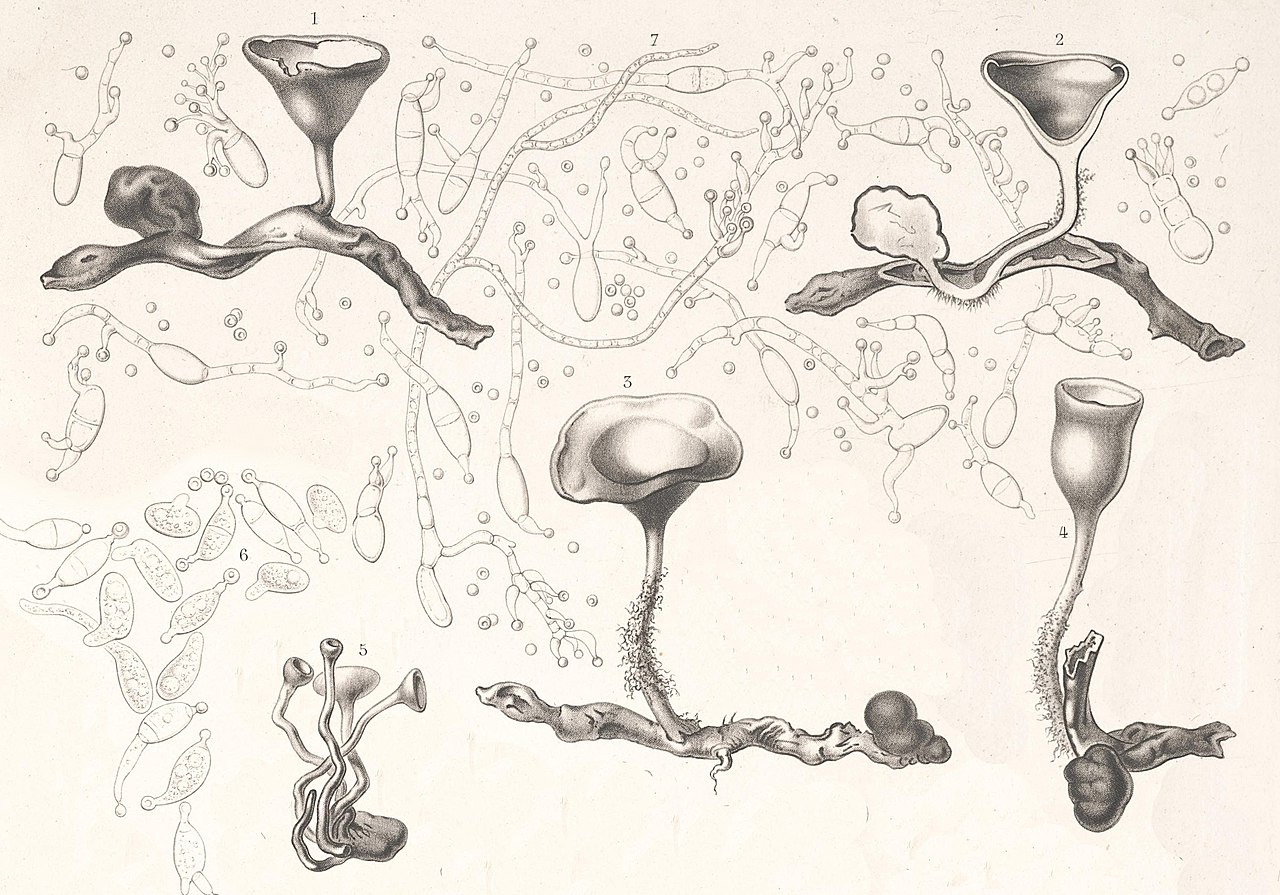
\includegraphics[width=\linewidth]{Figures/PezizaTuberosa.jpg}
%     \caption{Illustration of the fungus Dumontinia tuberosa by physician, mycologist, and illustrator Charles Tulasne (1816–1884) in the book Selecta Fungorum Carpologia (1861–65). (Name of the original work: Peziza tuberosa parasite on Anemone nemorosa).}
%     \label{fig:tcanther}
% \end{figure}

% \subsection{DCA for MSSC}
%example derivation of DC functions from MSSC. reference a few other versions. Point is to show that there are many DCA adaptations of MSSC 

% \subsubsection{Implented version}
%note sufficient versions, proof for rho, reference to T -- will not discuss much other than reference original material 

% \blindtext